\documentclass{article}

\usepackage[T1]{fontenc}
\usepackage[utf8]{inputenc}
\usepackage{lmodern}
\usepackage{amsmath}
\usepackage{graphicx}
\usepackage{bm}
\usepackage{fancyvrb}

\author{Sigrid Videm}
\title{Project 3}

\begin{document}
\maketitle
\tableofcontents % for a table of contents

\section{Abstract} 
I have used object oriented code and the Velocity Verlet method to model the movement of the planets of our solar system. It has been a battle between keeping the number of grid points low enough to simulate for many years of the future, and keeping the step length low enough to get stable solutions. I have found that the most vulnerable part is Mercury. Because of its short orbital period, I need more grid points if I want to include mercury in my simulations. I have been able to simulate the whole solar system for 50 years with a step length of $1/100$, and all planets exept mercury for 1000 years with step length $1/25$. That being said, in both cases, the precision of the solution for the planet with the shortest orbital period is poor. For most of the project, I have used the Velocity Verlet method, but I have also comapared the Velocity Verlet method to the Euler Cromer method. Euler cromer is faster, but the error is larger. 
I have devoted some extra time on the Earth-Sun system, and verified that the theoretical escape velocity and gravitational force give a stable solution.
\section{Introduction}
The aim of this project was to use object oriented code to model the movement of the planets of our solar system. All planets are governed by the Newtoninan gravitational force
 $$F_G=\frac{GM_{\odot}M_{\mathrm{Earth}}}{r^2}$$ 
and Newton's second law
$$
\bm{F}=m \frac{\textrm{d}^2 \bm{r}}{\textrm{dt}^2}$$
I rewrote the resulting second order differential equations to coupled first order differental equations. 

There are many methods for solving a first order equation, I have implemented the Euler Cromer method and the Velocity Verlet method.
The reason for using object orientation, is threefold. The force on each planet depends on the planets position relative to the other planets. This gives rise to many coupled differential equations. By implementing the planets as instances of a class, I only need to write the equations once, not a new set of equations for every planet. The second benefit is that it is easy to implement new solvers. In this project, I have used both the Euler Cromer method and the Velocity Verlet method, but if I want to try another solver, I can add it in the solver class. Third, but not less important, because I have made a class for the acceleration, I can use other interactions than the Newtonian gravitational force. Then it is possible to use the code to solve other many particle systems, such as a gas in a container, or many blocks connected with springs, or maybe to model neurons in a neural network.

First, I started out using the Euler Cromer method for modelling the cicular movement of Earth around the Sun, the other planets neglected. Here, I used a simplified expression for the acceleration. The theoretical background is presented in section 3.1, and a brief discussion on the quality of the results in 4.1. Then I started to write the code object oriented. How the code is structured, and  how I implemented the Velocity Verlet solver, is explained in section 3.2.1. In section 4.2.1, I investigate the conservation of energy and angular momentum, and look in the efficiency of the solvers. 
For me, the most exiting part of the project was to plot the motion of the planets. These plots are in section 4.2.4. 
In this work, I have only used two dimensions, because the planets lie almost in the same plane, I get nice plots, and because an extra dimension would require more run time. 
My code is available at https://github.com/sigrivi/Project3
\section{Methods}
\subsection{The circular orbit of Earth around the Sun}
The Earth-Sun system consists of a very massive Sun at a fixed position, and Earth, in a circular orbit around the Sun. The radius of the orbit, $r$, the speed, $v$, and the magnitude of the acceleration, $a$, will remain unchanged throughout the movement, because the only force acting on Earth is the gravitational force, which magnitude is constant when the radius is constant. The values of these constans are: 
$$r=1\textrm{AU}$$
$$v=\frac{2{\pi}r}{T} = \frac{2 \pi \cdot 1\textrm{AU}}{1 \textrm{yr}}$$
$$a=\frac{v^2}{r} = \frac{4{\pi}^2r}{T^2} = \frac{4 {\pi}^2 \cdot 1\textrm{AU}}{(1 \textrm{yr})^2}$$
When the orbit is circular, the acceleration vector always has the opposite direction of the position vector. This gives the the relation: 
$$a_x = -\frac{a}{r}x$$
$$a_y = -\frac{a}{r}y$$
where $(x,y)$ is the position of Earth when the Sun is situated in the origin, and $a_x$ and $a_y$ are the x and y-componets of the acceleration. For this spesific case, I used the Euler Cromer(\cite{EulerCromer}) method: 
$$v_{x,i+1} =v_{x,i} + h\cdot a_{x,i} = v_{x,i} - h\cdot \frac{a}{r}x_i$$
$$v_{y,i+1} =v_{y,i} + h\cdot a_{y,i}= v_{y,i} - h\cdot \frac{a}{r}y_i$$
$$x_{i+1} = x_i + h \cdot v_{x,i+1}$$
$$y_{i+1} = y_i + h\cdot v_{y,i+1}$$
$$h = \frac{t_{final}}{N}$$ 
$t_{final}$ is the time measured in years, $N$ is the number of grid points. I used the initial values $x=1, y=0, v_x=0, v_y=1$.
The code is found in project3a2.py, and produces a plot of a circular orbit. A plot where $t_{final}=1\textrm{yr}$ and $N=100$ is found in section 4.1. %To test the program, I checked whether the radius remains constant, the position and velocity are orthogonal, and the end point equals the starting point. The results are found in the Results and Discussion  section, along with a discussion of how these values depends on $h$. 

In general, the acceleration is not constant. My next step was to make a program which calculates the acceleration of Earth, based on the distance to the Sun. I chose to do this with an object oriented code, so that the addition of the other planets became straight forward. The method is described in the next paragraph. I did the further investigation of the Earth-Sun system with this program. You will find more exciting details about the Earth-Sun system under the captions Escape velocity (section 3.2.2) and The gravitational force (section 3.2.3). 

\subsection{The solar system}
\subsubsection{The model of the solar system}
I structured my code in the following way. The first class is a class for planets, the attributes for this class are mass, position, velocity, acceleration, name, a function which calculates the total(potential and kinetic) energy of the planet and a function which calculates the angular momentum. The second class is a class for acceleration. This class contains only one function, which updates the acceleration of a planet, using the positon and mass of the other planets. The reason for making a class for this function, is that it gives me the oppertunity to use another potential function, in  case I want to use the code to solve other kinds for many-particle systems. The third class is a class containing functions which are differential equations solvers. I wrote one function using the Euler Cromer method, and one using the Velocity verlet Method. The Euler Cromer method is equal to the previously described one, with the exception that the acceleration is calculated for every step. For every planet $i$, the total acceleration is a sum:
\begin{equation} \label{eqn1}
a_x=-\sum\limits_{j=0}^{N_p} \frac{GM_{\odot}}{r_{i,j}^2} \frac{x_{i,j}}{r_{i,j}}
\end{equation}
Where $r_{i,j}$ is the distance between planet $i$ and planet $j$, $x_{i,j}$ is the x-component of this distance. The same expression applies for the y-direction. I chose to make a two-dimensional model, but in my program all vectors are three-dimensional with the z-component equal to zero, so that the addition of a third dimension is possible.
Calculation of the acceleration is done by calling the Update function of the acceleration class. The Update function uses a list of planets as input, and alters the value of the acceleration. 
\begin{verbatim}
def Update(self, Planets):
		for k in range(3): ## 3 is the length of the r and v vector

			for i in range(self.N_p): #N_p is the number of planets in the list
				P = Planets[i]
				P.a[k] = 0
				for j in range(self.N_p):
					if j==i:
						P.a[k] = P.a[k] -4*pi**2*P.r[k]/np.linalg.norm(P.r)**3 # gravitational force from the Sun
						
					else: 
						distance = P.r-Planets[j].r
						P.a[k] = P.a[k] - distance[k]*Planets[j].mass/np.linalg.norm(distance)**3 #gravitational force from planet j
		return(Planets)

\end{verbatim}


I will now explain the Velocity Verlet method. 
The equation I need to solve $$\frac{d^2x}{dt^2}=a(x,t)$$ can be rewritten as two coupled first order differential equations:
$$\frac{dx}{dt} = v$$
$$\frac{dv}{dt} = a$$
$x(t)$ is discretized as $x(t_i)=x_i$, where $t_i =t_0 +h\cdot i$ and $h=\frac{t_{final}-t_0}{N}$. To get an expression for $x_i$, I use the Taylor expansion:
$$x_{i \pm h}  = x_i \pm hx_i^{(1)}+\frac{h^2}{2} x_i^{(2)}+O(h^3)=x_i \pm hv_i + \frac{h^2}{2}a_i +O(h^3)$$
$$x_{i + h}  \approx x_i + hv_i + \frac{h^2}{2}a_i$$
$$v_{i \pm h}  = v_i \pm hv_i^{(1)}+\frac{h^2}{2} v_i^{(2)}+O(h^3) = v_i \pm ha_i + \frac{h^2}{2} v_i^{(2)}+O(h^3)$$
I found $v_i^{(2)}$  by Eulers formula: 
$$hv_i^{(2)}=v_{i+1}^{(1)}-v_i^{(1)}$$
$$v_{i + h} = v_i + ha_i + \frac{h}{2} (v_{i+1}^{(1)}-v_i^{(1)})+O(h^3)= v_i + ha_i + \frac{h}{2}(a_{i+1}-a_{i})+O(h^3)$$
I want an apprximate value for $v_{i+1}$:
$$v_{i+1} \approx v_i + \frac{h}{2}a_{i+1}+\frac{h}{2} a_{i}$$
Because $a_i$ depends on $r_i$, and $a_{i+1}$ depends on $r_{i+1}$, I devided the calculation of $v_{i+1}$ in two half steps, as shown in the code below. 
\begin{verbatim}
def VelocityVerlet(self,Planets):
		h = self.h
		for P in Planets:
			for i in range(len(P.v)):
				P.v[i] = P.v[i]+0.5*h*P.a[i]
				P.r[i] = P.r[i]+h*P.v[i]
		accel = Acceleration(Planets)
		accel.Update(Planets)
		for P in Planets:
			for i in range(len(P.v)):
				P.v[i] = P.v[i]+0.5*h*P.a[i]
\end{verbatim}
I made a solve function which uses the Update function and either the EulerCromer or the VelocityVerlet. Solve returns two arrays, x and y, which contains the calculated positions of all the planets. The classes and the solve function are found in $project3b.py$  
To compare the solvers, I made CompareSolvers, a function which makes two planet lists containing only the Earth. It calculates and plots the relative difference in total energy and angular momentum of the starting point and the end point, depending on h. A log-log plot of relative difference in total energy against step length is presented in section 4.2.1. I had some surprising results regarding the angular momentum, these are also presented there. The code is in project3c.py. 


I counted the number of FLOPs for the Euler Cromer method : $$number of planets \times dimension \times 4 \times N$$
and the number of FLOPs for the velocity Verlet method:
$$number of planets \times dimension \times 8 \times N$$
With one planet and two dimensions this gives $64N$ FLOPs for Euler Cromer, and $128N$ FLOPs for the Velocity Verlet. The Euler cromer should be twice as fast as the Velocity Verlet for the same number of discretization points.
\subsubsection{Escape velocity}
For the initial velocity of Earth, I have used $v_y=2\pi \textrm{AU} / \textrm{yr}$, because this is the velocity of an object in a circular orbit with a period of $1 \textrm{yr}$ and a radius $1 \textrm{AU}$. The theoretical escape velocity is when the total energy of the Earh is zero:
$$\frac{1}{2}mv^2=\frac{GMm}{r}$$ 
$$v= \sqrt{\frac{2GM}{r}}= \sqrt{ \frac{2\cdot 4 {\pi}^2 \cdot (1\textrm{AU})^2}{(1 \textrm{yr})^2}}$$
The escape velocity is $v=2 \sqrt{2}\pi \textrm{AU} / \textrm{yr}$. I plotted the orbit of Earth for initial velocities $v=2\pi, 2.5\pi, 2 \sqrt{2}\pi, 3\pi, 3.5\pi$, and calculated the total energy(See section 4.2.2). 
The code for exploring the escape velocity is in project3d.py.
\subsubsection{The gravitational force}
The gravitational force on Earth from the Sun is $$
F_G=\frac{GM_{\odot}M_{\mathrm{Earth}}}{r^2},
$$
What would happen if the force decayed more rapid with the distance between Earth and the Sun? I've made a plot( figure \ref{fig:gravitationalForce}) exploring this, using  
\[
F_G=\frac{GM_{\odot}M_{\mathrm{Earth}}}{r^{\beta}},
\]
where $\beta\in [2,3]$. The way I implemented this in my code, was to make an additional variable in the Update function. The default value is 3 (see Equation \ref{eqn1}). 
\begin{verbatim}
def Update(self, Planets, beta = 3.):
\end{verbatim}
The code for exploring the gravitational force is in project3d.py.

\subsubsection{All the planets of the solar system}
To model the movement of all the planets of the solar system, I made one instance of the Planet class for every planet. I found the planet masses in the  in the project description\cite{Projectdescription}, and calculated planet masses measured in solar masses. I got the initial positions and initial velocities for the NASA website \cite{NASA}. I chose to use only two dimensions, so all the z-components were set to zero. I made a plot function, where you can choose the distance in time between the points in the plot. This part of the code is in project3f.py.  In section 4.2.3, there are plots of the whole system for different values of $t_{final}$, and a short discussion of the stability of the system.  

\subsubsection{The perihelion precession of Mercury}
The orbit of mercury has a precession of its perihelion (the point where Mercury is closest to the Sun). This is due to the influence of the other planets, and to the relativistic effect. I want to study the relativistic effect. Therefore, I will only look at the Mercury-Sun system. According to classical theory, the perihelion will be a fixed point. Including the relativistic effect, the force on Mercury from the Sun is
\[
F_G = \frac{GM_\mathrm{Sun}M_\mathrm{Mercury}}{r^2}\left[1 + \frac{3l^2}{r^2c^2}\right]
\]
I implemented this in the Update function. If the planet's name is Mercury, the relativistic expression is used, else the Newtonian expression for the gravitational force. According to the project description \cite{Projectdescription}, the perihelion angle $\theta_p = \frac{y_p}{x_p}$ should have a precession of 43 arcsecs per century. In order to find such a small deviation, I need very high resolution. An estimate for the necessary number of grid points is about $360\cdot 60\cdot 60\cdot 4\cdot 100 = 518400000$ (degrees in a circle $\times$ seconds in a degree $\times$ number of mercury orbits per year $\times$ years in a century). I need to run the Mercury-Sun simulation for $h=1/5184000$ and $t_{final}=100$. Then, I need a loop which goes through the first $5184000/4$ elements of the solution vectors and the $5184000/4$ last and finds the minimum distances to the sun (First and last Mercury year of the century). Then, I need to calculate $\theta_p$ for both $r$, and compare the two. Because my code is not nearly efficient enough, I have not done this. A estimates of run time is found in section 4.2.5. project3g.py is a sketch of how I would write my code if I set out to do so. 
\section{Results and Discussion}
\subsection{The circular orbit of Earth around the Sun}
Figure \ref{fig:earth-sun} shows the path of Earth in orbit around the Sun. The radius of the circle is 1 AU. I made the plot with a Euler Cromer discretization specialized for the case of circular orbit. The step lenght $h=1\textrm{yr}/100 \approx 4 \textrm{days}$. I tried different step lengths. The end point deviation, $(x_0-x_N,y_0-y_N)$ is small, and decreases by a factor $10^{-3}$ as $h$ decreases by $1/10$. The same does the squared speed deviation: $v_0^2-v_N^2$. This means that for one orbit around the sun, you don't need too many grid points to get both potential energy and kinetic energy to be preserved. The radius deviation, which is the max of $x_i^2 +y_i^2-r^2$ and the maximum deviation from orthogonality $x_i\cdot v_{x,i}+y_i \cdot v_{y,i}$ decrease proportionally to h. See Table \ref{tab:table1} for details.

\begin{figure}
  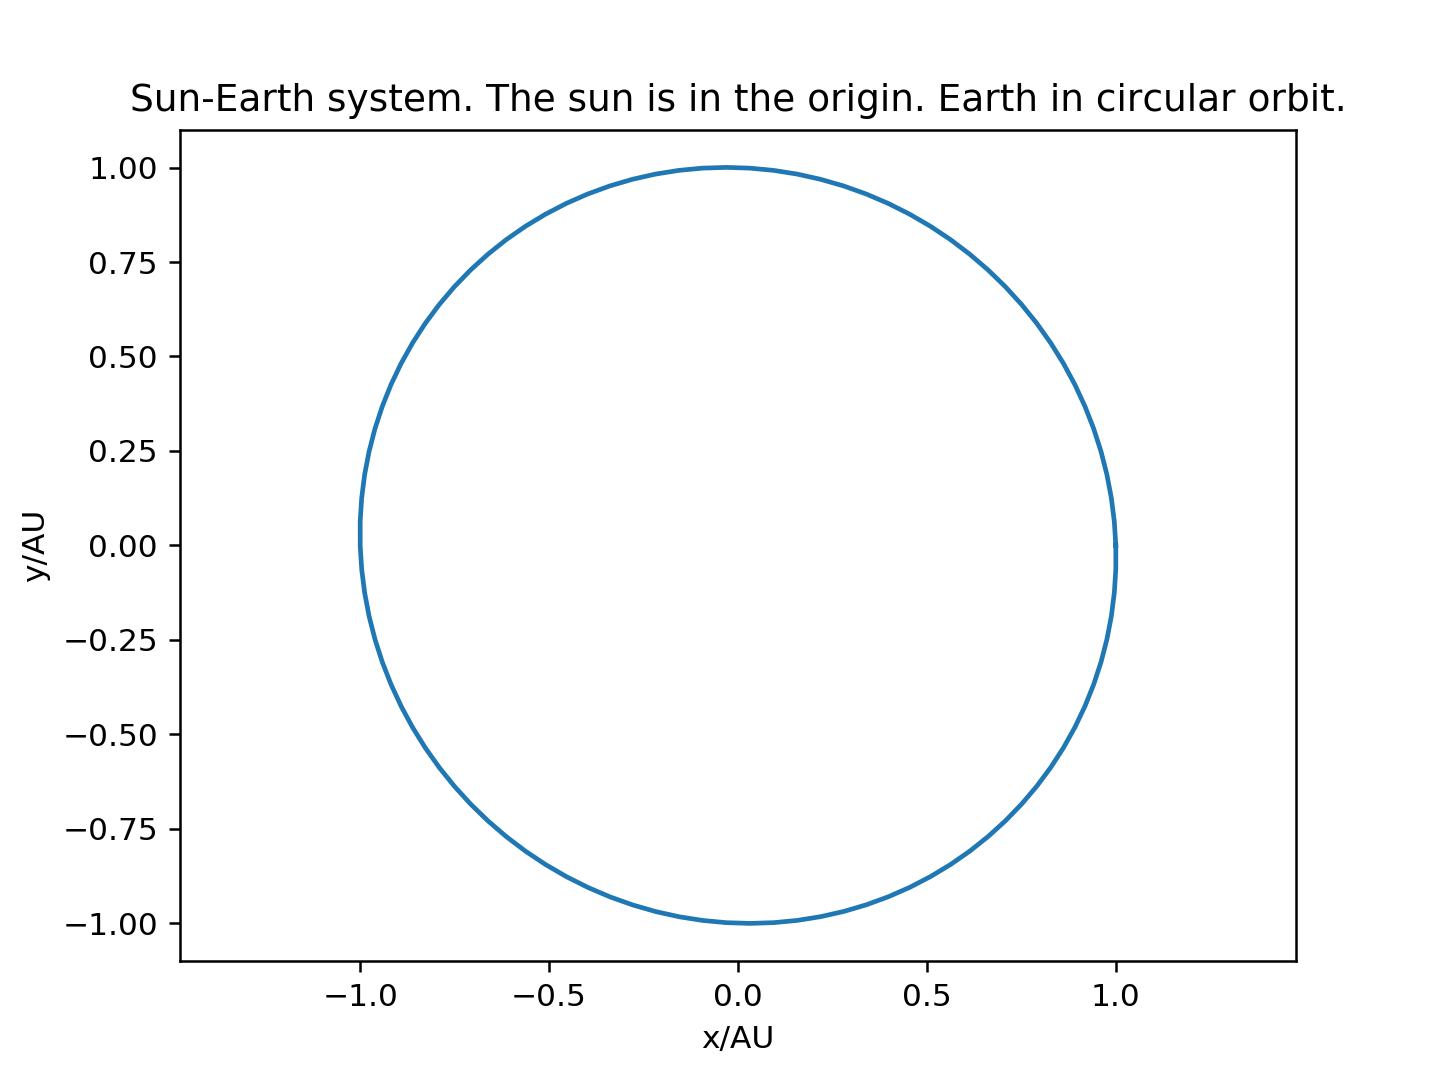
\includegraphics[width=\linewidth]{sun_earth.png}
  \caption{Earth in circular orbit around the Sun. One year. Step length approximately 4 days}
  \label{fig:earth-sun}
\end{figure}

\begin{table}[h!]
  \centering
  \caption{Quality of the solution depending on $h$}
  \label{tab:table1}
  \begin{tabular}{l||l|l|l|l|}
   $h$  & end point  & radius   & orhogonality   & squared speed \\ 
        &   deviation &   deviation &   deviation &  deviation\\ 

    \hline
    1/100  & 3.30e-05 -1.03e-03 & 3.24e-02 & 3.95e-01 &  -2.56e-03\\
    \hline
    1/1000 & 3.25e-08 -1.03e-05 & 3.15e-03 & 3.94e-02 & -2.56e-06 \\
    \hline
     1/10000 & 3.24e-11 -1.03e-07 & 3.14e-04 & 3.94e-03 & -2.56e-09
\\
	\hline
	1/100000 & 3.47e-14 -1.03e-09 & 3.14e-05 & 3.94e-04 & -2.01e-12
\\
  \end{tabular}
\end{table}
The method gives good results for the end point. With $h=1/100$ both position and speed is the same at $t_0=0$ and $t_{final} = 1 \textrm{yr}$ with 3 leading digits. Because the end point values are good, the method is suited for simulations with duration of more than one year, but for many years, the deviation will accumulate. Also, if you want to run it for many years with the same step length, you need more grid points, and the run time will be long.  However, the maximum radius deviation is larger, this means that the orbit is not entirely circular. The orthogonality deviation seems to be about one order of magnitude larger than the radius deviation.
%Also, since the velocity and the radius are not orthogonal, this method cannot be used to calculate the speed at other points than the end point. WHY?
\subsection{The solar system}
\subsubsection{The model of the solar system}
\begin{figure}
  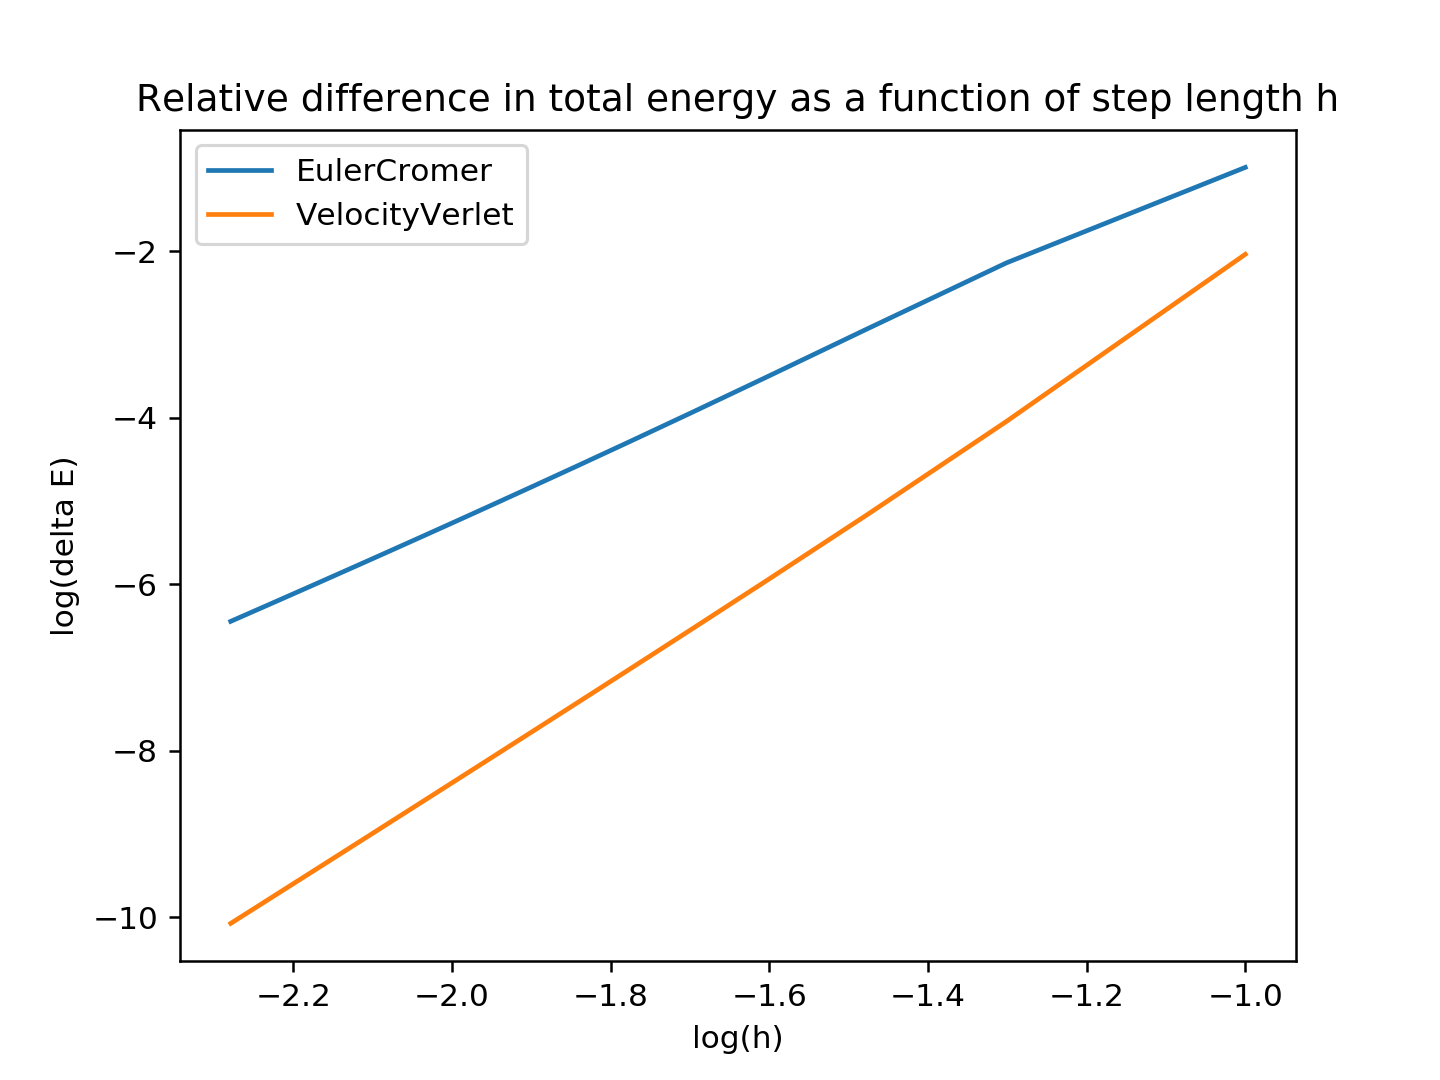
\includegraphics[width=\linewidth]{energy_loss.png}
  \caption{Relative difference in total energy after one year as a function of step length h with the Euler Cromer solver and the Velocity Verlet solver. The slope of the orange line is 6.3, the slope of the blue line is 4.3}
  \label{fig:energy_loss}
\end{figure}
To compare the Euler Cromer and the Velocity Verlet, I calculated the total energy at the starting point $t=0$ and the end point $t_{final} =1 \textrm{ yr}$ for different step lengths. I calculated the relative difference in energy between the starting point and the end point:
$$\Delta E = \frac{E_{initial}-E_{final}}{E_{initial}}$$
The results are presented as a log-log plot, se figure \ref{fig:energy_loss}. The slope of the Velocity Verlet error devided by that of Euler Cromer is $6.3/4.3 \approx 3/2$. I will show that the ratio is the expected one: The error of the Euler Cromer method, $\epsilon_E$, is proportional to $h^2$, while the error of the Velocity Verlet, $\epsilon_V$, is proportional to $h^3$ (because we leave out terms of $O(h^2)$ and higher in the Euler Cromer method, and leave out terms of $O(h^3)$ and higher in the Velocity Verlet method). 
$$\epsilon_V \propto h^2$$
$$\epsilon_E \propto h^3$$
$$\log \epsilon_V  \propto \log h^2 = 2\log h$$
$$\log \epsilon_E  \propto \log h^3 = 3\log h$$
$$\frac{\epsilon_V}{\epsilon_E} = \frac{3}{2}$$

My input data(the mass of the planets) has a precicion of three leading digits, so I am content with an error of magnitude $10^{-4}$. To get an error of this magnitude with Euler Cromer, I need $h=10^{-1.8}\approx 1/60$, while with Velocity Verlet it is sufficient with $h=10^{-1.3}\approx 1/20$. For the rest of this project, I used the Velocity Verlet solver. Becuase most of the plots are made with a small $t_{final}$, run time was not an issue, and I used $h=1/100$. This gives an error of magnitude $10^{-8}$. 


I also calculated the angular momentum $\bm{L} = \|\bm{r} \times \bm{p}\|$ at the starting point and at the end point. To my suprise, this value remained constant, even at very large step lengths. I thougth this had someting to do with the end points, so I printed the values of $r$, $v$ and $\|\bm{r} \times \bm{v}\|$ for every step, by including a print command inside the solve function. The results for $h=1/10$, $t_{final} = 1 $ are shown in the tables \ref{tab:table2} and \ref{tab:table3}. Both radius and velocity changes, but it seems like both the Velocity Verlet and the Euler Cromer conserves the angular momentum.   I have not studied this quantity for a system with more planets.%, but I guess that this effect is unique for the circular movement. 
\begin{table}[h!]
  \centering
  \caption{The radius and velocity at point nr. N in the simulation, using the Velocity Verlet solver with $h=1/10$, $t_{final} = 1 $}
  \label{tab:table2}
  \begin{tabular}{l||l|l|l|l}
grid point & radius & velocity & radius$\times$velocity \\
\hline
1. & 1.01929565702 & 6.17846064977 & 6.28318530718 \\
2. & 1.06722313673 & 5.91980428907 & 6.28318530718 \\
3. & 1.12253534997 & 5.62649166547 & 6.28318530718 \\
4. & 1.16621308296 & 5.39988748354 & 6.28318530718 \\
5. & 1.18671335125 & 5.29513506661 & 6.28318530718 \\
6. & 1.17951052497 & 5.33182329181 & 6.28318530718 \\
7. & 1.14613513838 & 5.50347805201 & 6.28318530718 \\
8. & 1.09454769405 & 5.77407563779 & 6.28318530718 \\
9. & 1.04027469647 & 6.06486626165 & 6.28318530718 \\

  \end{tabular}
\end{table}

\begin{table}[h!]
  \centering
  \caption{The radius and velocity at point nr. N in the simulation, using the Euler Cromer solver with $h=1/10$, $t_{final} = 1 $}
  \label{tab:table3}
  \begin{tabular}{l||l|l|l|l}
grid point & radius & velocity & radius$\times$velocity \\
\hline
1. & 0.872393471784 & 7.4205034984 & 6.28318530718 \\
2. & 0.895594719456 & 7.96473693791 & 6.28318530718 \\
3. & 1.04943612094 & 7.10949959888 & 6.28318530718 \\
4. &1.22992078748 & 5.99238483753 & 6.28318530718 \\
5.& 1.38018921984 & 5.13525305666 & 6.28318530718 \\
6.& 1.48220853616 & 4.56253244426 & 6.28318530718 \\
7 & 1.53109412233 & 4.24048808256 & 6.28318530718 \\
8.& 1.52573981123 & 4.14966591817 & 6.28318530718 \\
9. & 1.46623678223 & 4.2852886316 & 6.28318530718 \\

 \end{tabular}
\end{table}

In the same simulation as I used for the error plot (figure \ref{fig:energy_loss}), I also printed the run times, see table \ref{tab:time}. The data in table \ref{tab:time} confirms the predidiction that the Euler Cromer run time is half the run time of the Velocity Verlet, becuase the ratio between the two is approximately 2. Also, the run time of both solvers is proportional to $N$. 
\begin{table}[h!]
  \centering
  \caption{Run time with Euler Cromer and with Velocity Verlet as a function of grid points(N). Last column is the ratio between these run times.  }
  \label{tab:time}
  \begin{tabular}{l||l|l|l|l}
N & Euler Cromer & Velocity Verlet & ratio \\
\hline
10 &0.00032 & 0.00064 &1.98 \\
20 &0.00053 & 0.00107 &2.02 \\
30 &0.00126 &0.00166 &1.31 \\
40 &0.00139 &0.00294 &2.12 \\
50 &0.00170 &0.00340 &1.99 \\
\hline
100 & 0.00245 &0.00477 &1.94 \\
\hline
150 &0.00364 &0.00757 &2.08\\
160 &0.00391 &0.00779 &1.99\\
170 &0.00425 &0.01031 &2.42\\
180 &0.00433 &0.00882 &2.03\\
190 &0.00546 &0.01055 &1.93\\

 \end{tabular}
\end{table}


\subsubsection{Escape velocity}
I plotted the orbit of Earth for inital velocities $v=2\pi, 2.5\pi, 2 \sqrt{2}\pi, 3\pi, 3.5\pi$. The first plot has $t_{final} = 1\textrm{yr}$, the second  $t_{final} = 3\textrm{yr}$, to see how the orbit evolves over time. For both plots I used h=1/100. 

Figure \ref{fig:oneyear} and \ref{fig:threeyear}  illustrate that initial velocities smaller than  $\sqrt{2}\cdot2\pi$ produces closed orbits. This is consistent with the theoretical value. With larger or equal inital velocity, Earth escapes the graviational field of the Sun. I calculated the initial total energy for each initial velocity. The calculated initial energies are 
$$E(2\pi)=-5.92e-05$$
$$E(2.5\pi)=-2.59e-05$$
$$E(\sqrt{2}\cdot2\pi) = 0.0$$
$$E(3 \pi) = 1.48e-054$$
$$E(3.5\pi)= 6.29e-05$$
The total energy corresponding to the escape velocity is zero, as predicted.  
\begin{figure}
  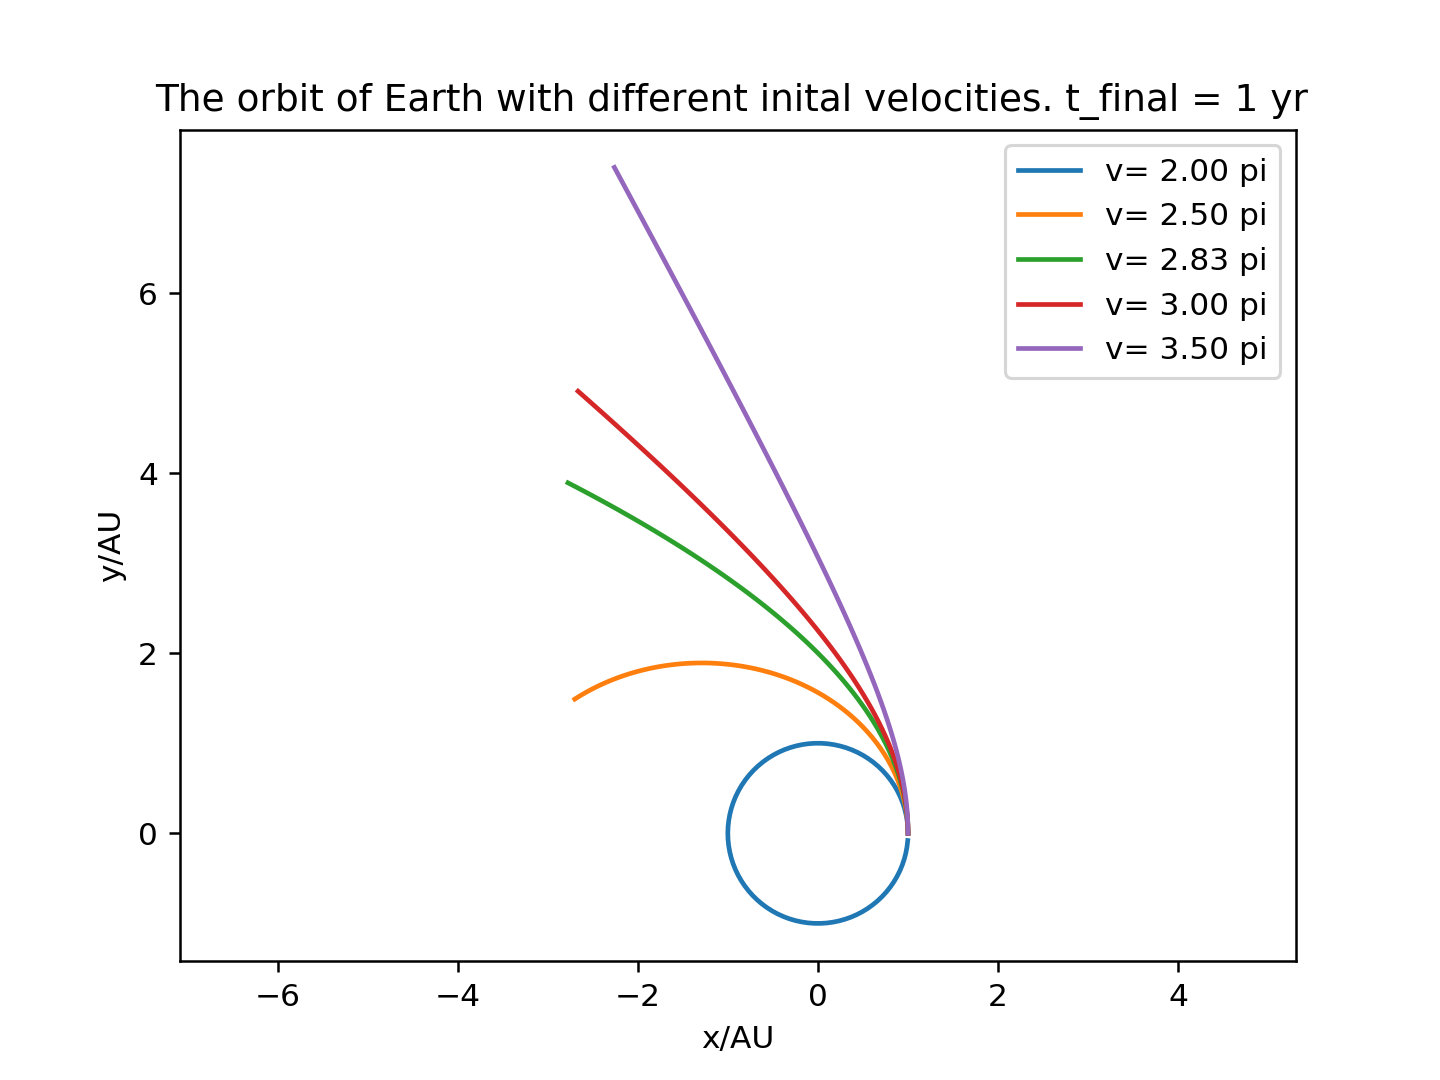
\includegraphics[width=\linewidth]{oneyear.png}
  \caption{One year of the movement of Earth around the sun with different initial velocities. Inital velocity $2\pi$ gives a circular orbit.}
  \label{fig:oneyear}
\end{figure}

\begin{figure}
  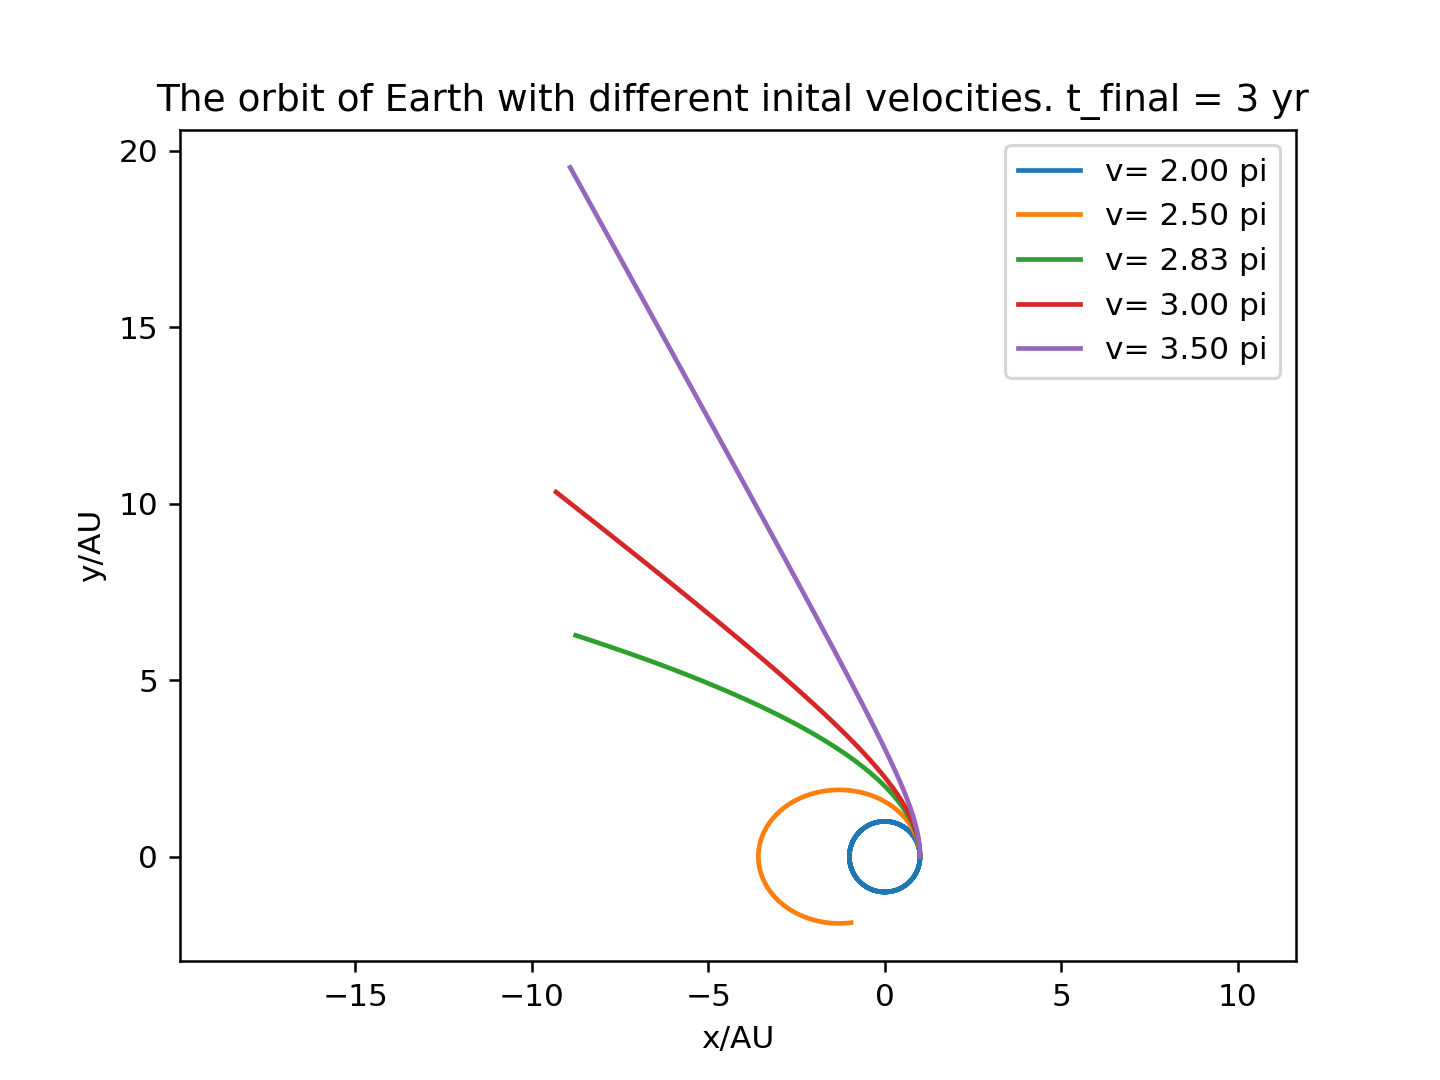
\includegraphics[width=\linewidth]{threeyear.png}
  \caption{Three years of the movement of Earth around the sun with different initial velocities.Inital velocity $2\pi$ gives a circular orbit. Inital velocity larger or equal to $2 \sqrt{2}\pi$ results in an unstable system.}
  \label{fig:threeyear}
\end{figure}

\subsubsection{The gravitational force}
The gravitational force decreases proportionally to  $ \frac{1}{r^2}$.  Figure \ref{fig:gravitationalForce} seems to indicate that with $\beta =2.5$, keeping the initial velocity unchanged, Earth still have a circular orbit, but when $\beta =3$, the gravitational force is not strong enough to keep Earth in orbit, and Earth sprials away. (Note that in the code, $\textnormal{beta} \to \beta+1$, as accounted for in equation \ref{eqn1})

\begin{figure}
  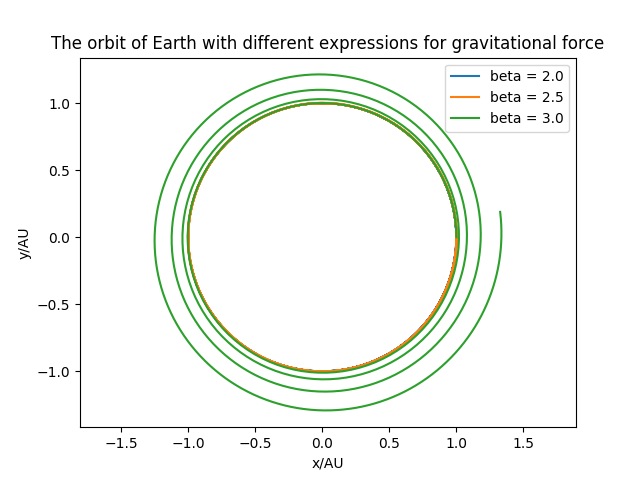
\includegraphics[width=\linewidth]{gravitationalForce.png}
  \caption{The orbit of Earth around the sun when the gravitational force is $F_G=\frac{GM_{\odot}M_{\mathrm{Earth}}}{r^{\beta}}$, plotted with $t_{final} = 5$. $F_G=\frac{GM_{\odot}M_{\mathrm{Earth}}}{r^{3}}$ results in an unstable system.}
  \label{fig:gravitationalForce}
\end{figure}
\subsubsection{All the planets of the solar system}
Figure \ref{fig:solar_system2} shows a close-up on the four innermost planets of the solar system. The center-of-mass is in the origin. I used $t_{final} = 2 \textrm{yr}$, because this is approximates the orbital period of Mars. During this period, Earth circles the Sun twice, Venus makes three rounds, and Mercury makes eight rounds. From my point of view, there are two intresting things about this plot. First, Earth has not the same center of its orbit as the other planets. I do not know why, but I believe it has to do with the initial positions. Second, the orbit of Mercury changes. I think this is a joint effect. Mercury has a shorter period and needs higher precision for the solution to be well-defined. Also, we know that the orbit of Mercury rotates around the focal points of the ellipse, and what we see in figure \ref{fig:solar_system2} migth have something to do with the shape of Mercury's orbits..
\begin{figure}
  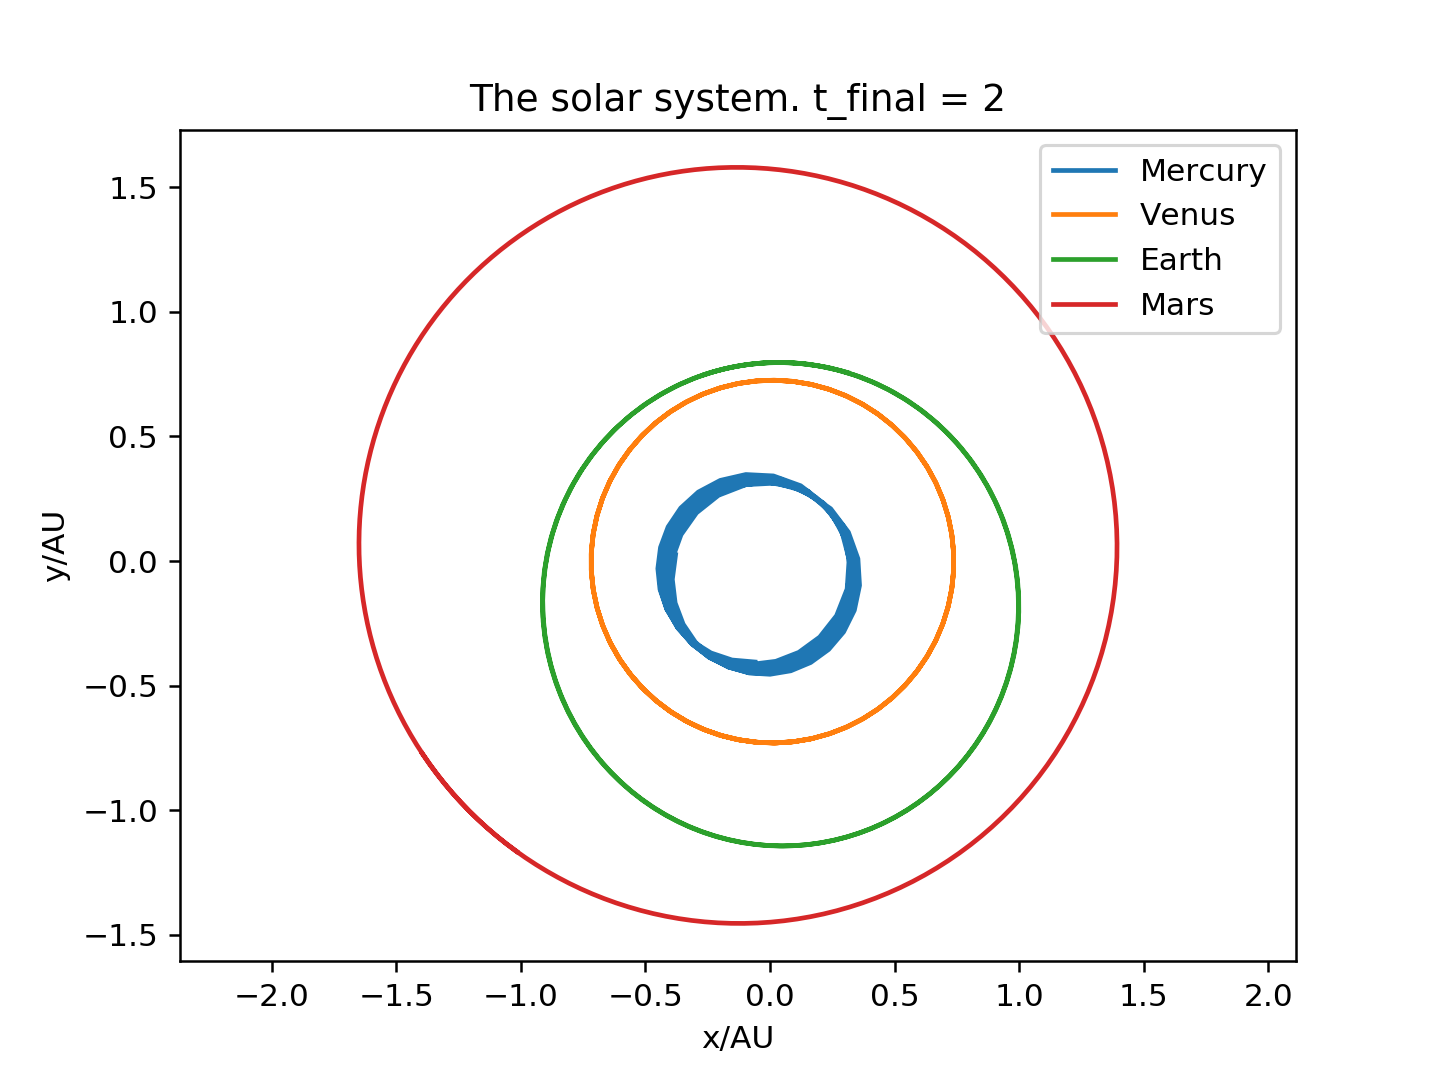
\includegraphics[width=\linewidth]{solar_system2.png}
  \caption{The orbits of the innermost planets in the solar system for the next 2 years. Mars, Earth and Venus have well-defined solutions, for Mercury, the precision is too low.}
  \label{fig:solar_system2}
\end{figure}

Figure \ref{fig:solar_system20} and \ref{fig:solar_system50} shows the orbits of all the planets of the solar system, calculated for 20 and 50 years from now.   These figures illustrates that both Uranus and Neptune have longer orbital periods than 50 years, but both have a curvature that indicates that the orbits are elliptic. Also, the orbits of the other planets seems stable. None of the planet's orbits are crossing, and, at least on this scale, there are no spirals. 

 
\begin{figure}
  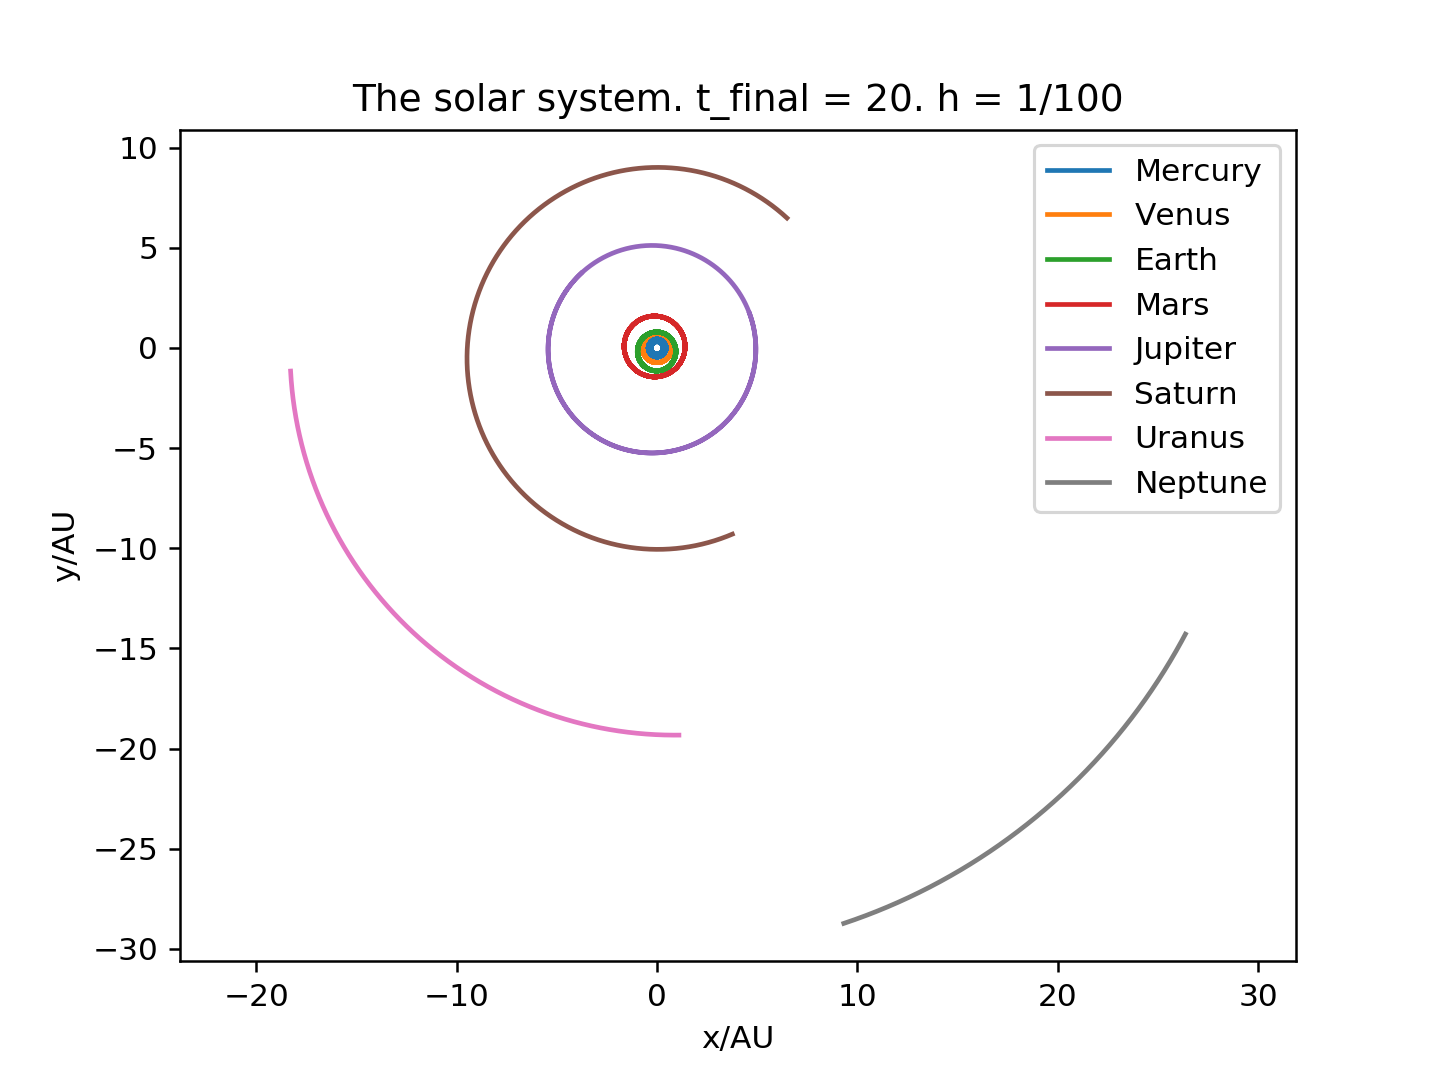
\includegraphics[width=\linewidth]{solar_system20.png}
  \caption{The orbits of the planets in the solar system for the next 20 years.}
  \label{fig:solar_system20}
\end{figure}

\begin{figure}
  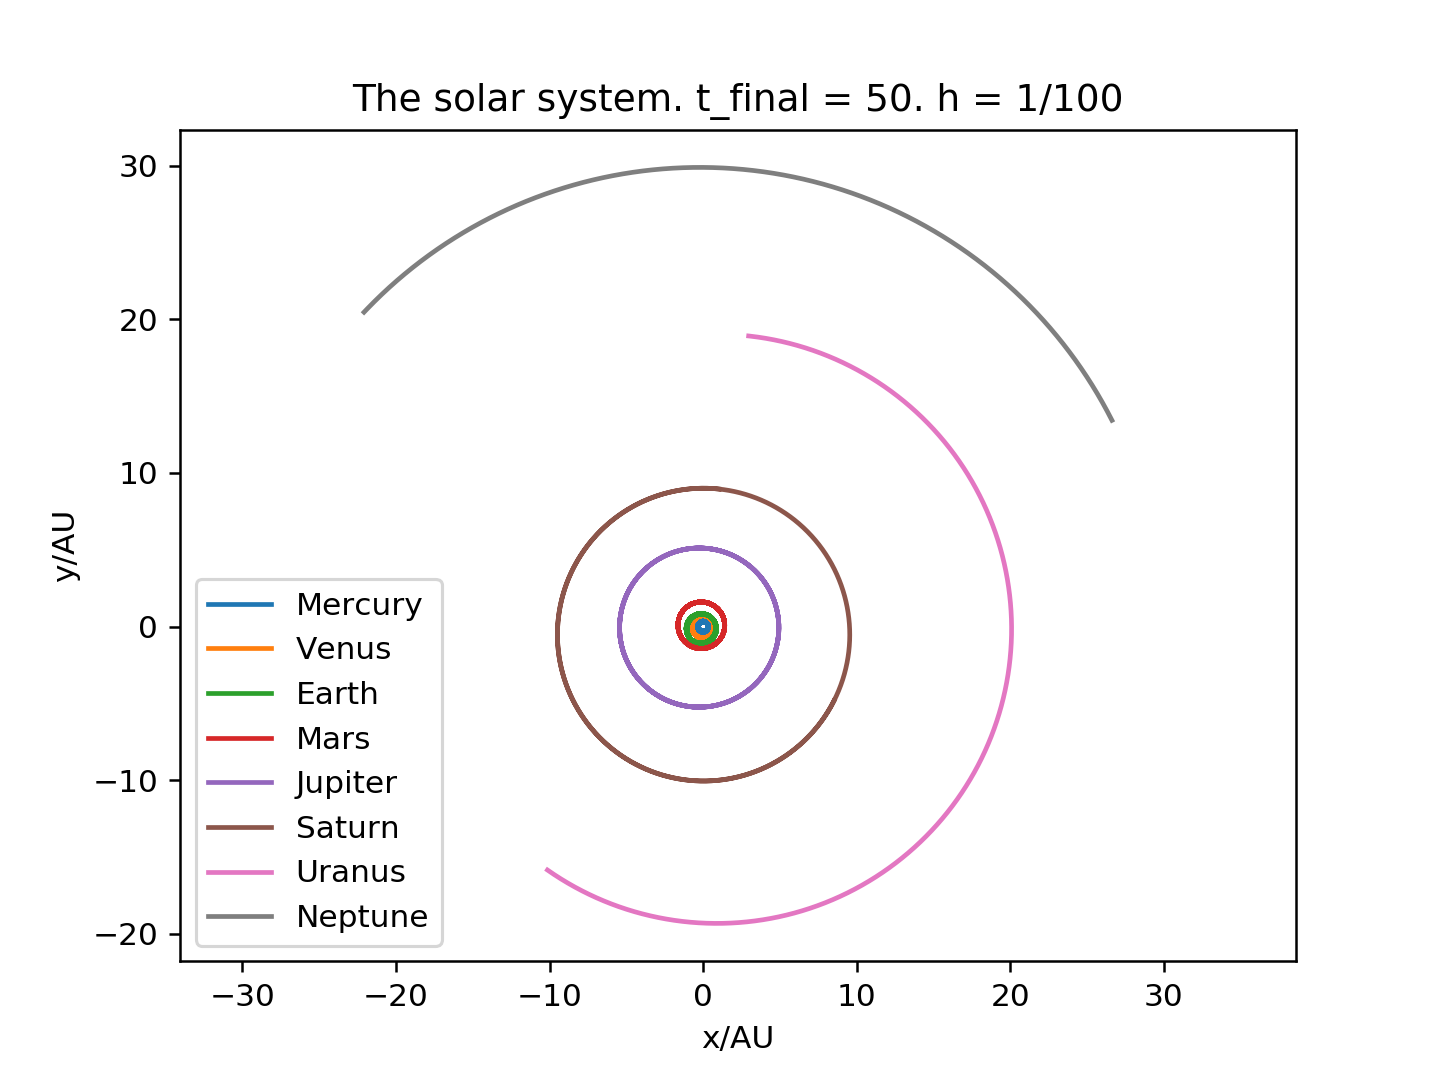
\includegraphics[width=\linewidth]{solar_system50.png}
  \caption{The orbits of the planets in the solar system for the next 20 years.}
  \label{fig:solar_system50}
\end{figure}
To further investigate the stability of my code, I used $h=1/25$, and $t_{final}=1000\textrm{yr}$. Figure \ref{fig:solar_system1000} shows that on this time scale, the system is not stable. Mercury escapes the system, but all the orher planets stay in their orbit, although the orbits of the inner planets are not well-defined (This is not possible to observe on the figure, the resolution is not good enough, you have to run the program yourself.) The result was the same with and without the relativistic correction of the gravitational force on Mercury. I tried with smaller $t_{final}$, and discovered that the problem is the step length. The step length I found by studying the error plot in \ref{fig:energy_loss} is suitable for the orbit of Earth, but not for Mercury, whose orbit has a shorter period. In figure \ref{fig:solar_systemNoMercury}, I used the same $h$ and $t_{final}$, but excluded Mercury. In this case, the system is still stable, but the inner planets have more deviaton in their orbit. Maybe they will suffer the same fate as Mercury, if $t_{final}$ is even larger. For fun, I also tried to use the Euler Cromer solver for this case. It takes less time, and produces a plot similar to the one in figure \ref{fig:solar_systemNoMercury}. You should try it yourself. 

Simulations with all the planets takes a lot of time. I measured the run time when $t_{final}=20\textrm{yr}$ to be approximately 51s, and when $t_{final}=50\textrm{yr}$, it was 238s. The run time of Velocity Verlet with one planet for $N=100$ was 0.00477s. This run time did not include the acceleration update. The run time of the Velocity Verlet is proportional to $$number of planets \times dimension  \times N$$
With the acceleration update

$$(number  of planets)^3 \times dimension^2  \times N$$
The estimated run time values are: 
$$0.00477s \cdot 8^3 \cdot 2 \cdot 20=97.6896s$$
$$0.00477s \cdot 8^3 \cdot 2 \cdot 50=244.224s$$
which are of the same magnitude as the run times measured. This means, that if you want to run the simulation for $t_{final}=1000\textrm{yr}$ and $h=1/100$ with the aspiration of having Mercury in its place, it will take about
$$0.00477s \cdot 8^3 \cdot 2 \cdot 1000=4884.48s \approx 1.4 \textrm{hours}$$

\begin{figure}
  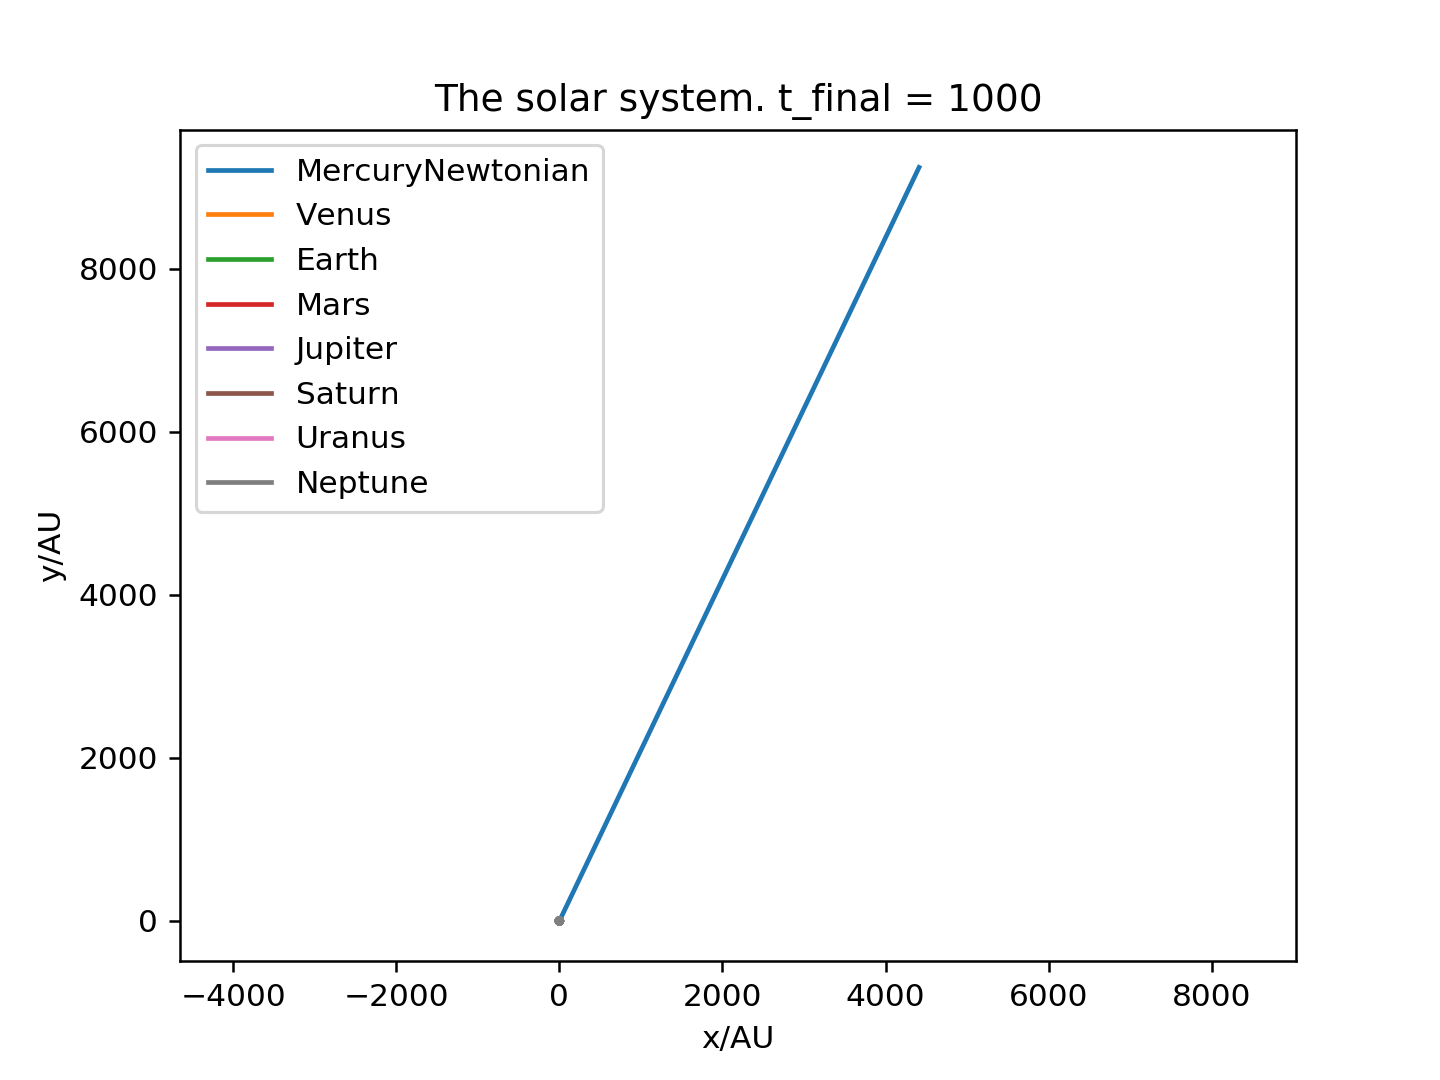
\includegraphics[width=\linewidth]{solar_system1000Newtonian.png}
  \caption{The orbits of the planets in the solar system for the next 1000 years.}
  \label{fig:solar_system1000}
\end{figure}

\begin{figure}
  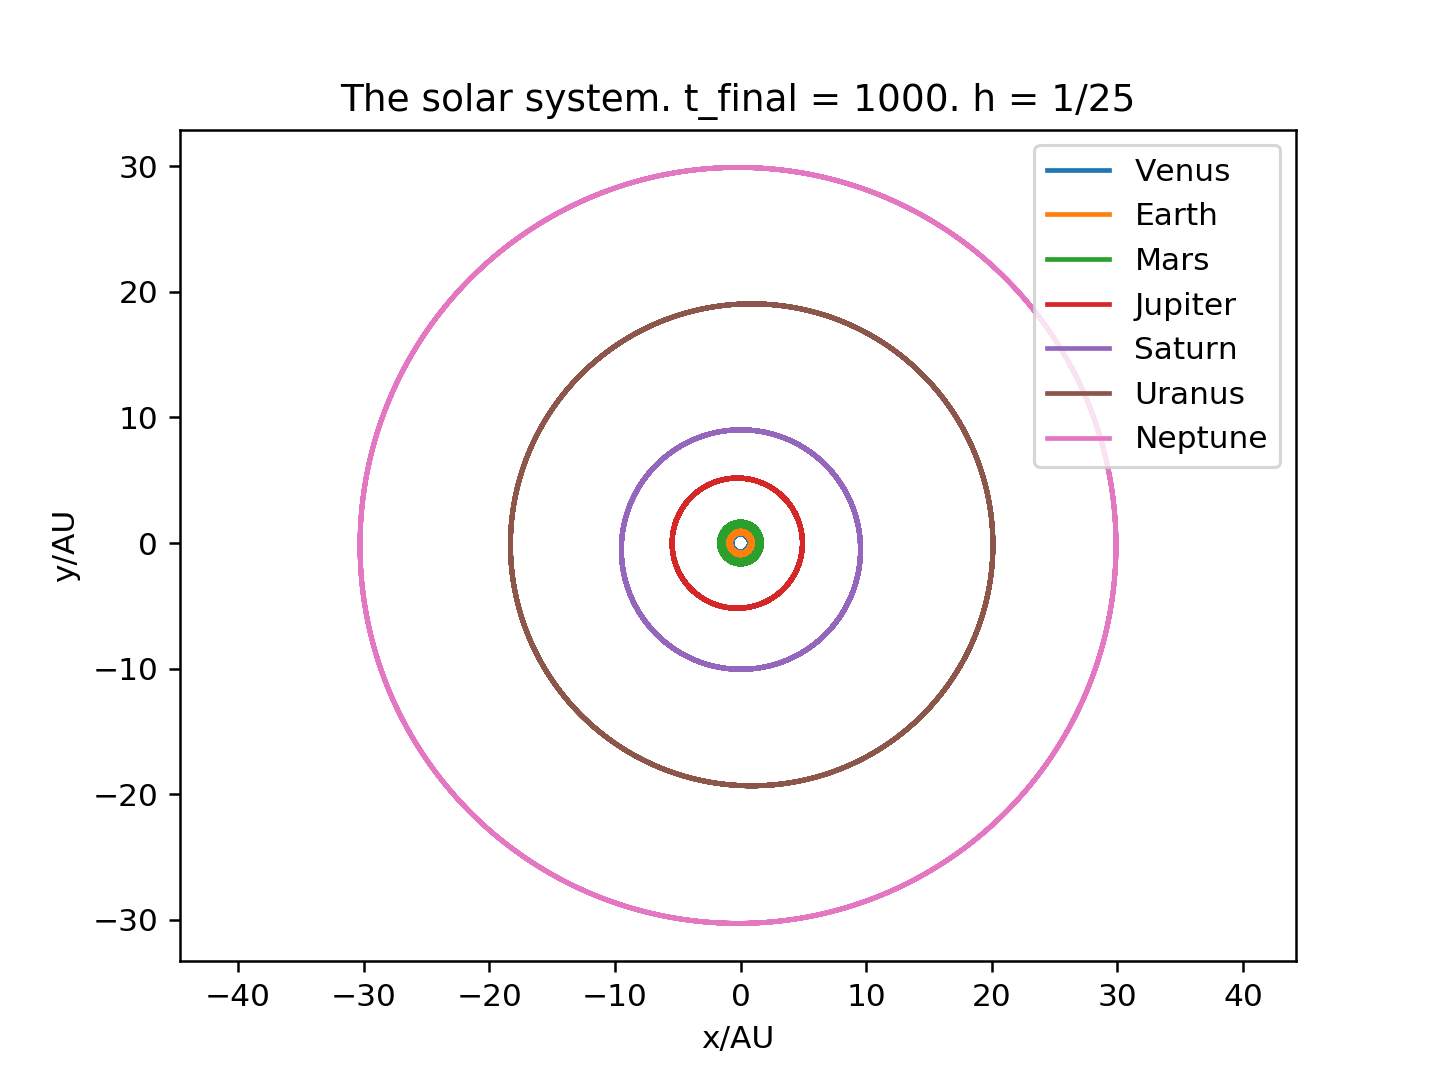
\includegraphics[width=\linewidth]{solar_systemNoMercury.png}
  \caption{The orbits of the planets in the solar system for the next 1000 years.}
  \label{fig:solar_systemNoMercury}
\end{figure}

\subsubsection{The perihelion precession of Mercury}

The simulation will take about: 
$$0.00477s \cdot 1^3 \cdot 2^2 \cdot 518400000 = 9891072 s  \approx 114 \textrm{days} $$
To do this part of the project, I have to rewrite my code so that it becomes more efficient. Hopefully, that would take less than 114 days, but still it will take more time than what is left before the deadline. 
\section{Conclusion}
I have seen that rewriting second order differental equations into coupled first order differtial equations, and using the Velocity Verlet method to solve these equations, is a good approach to the Earth-Sun system. With object orientation, it is easily extended to include many planets. The Euler Cromer method is two times faster than the Velocity Verlet, but needs more grid points in order to maintain energy conservation. The step length and the the number of years you want to simulate, affect the quality of the solution. Planets with a short orbital period, needs a smaller step length. 


Furter work will involve the investication of why the solvers conserves the angular momentum(the exact quantity). I want to find out if this propery is unique for circular motion of only one planet, or if it applies to the other planets as well. I also want to do a more systematic evaluation of how many grid points that are neccessary, depending on $t_{final}$ and the planet of choise. 
\begin{thebibliography}{1}

\bibitem{Projectdescription} 
Hjort-Jensen, M.: Computational Physics: Project 3,
\\\texttt{http://compphysics.github.io/ComputationalPhysics/doc/Projects/2017/Project3/html/Project3.html}

\bibitem{EulerCromer}
Wikipedia: The Euler Cromer method,
\\\texttt{https://en.wikipedia.org/wiki/Semi-implicit\_ Euler\_ method}

\bibitem{NASA}
NASA: HORIZONS Web-Interface,
\\\texttt{https://ssd.jpl.nasa.gov/horizons.cgi}

\end{thebibliography}
\end{document}